\documentclass[12pt]{article}
\usepackage{../../ficha}

\begin{document}

\ficha{Ângulos na Circunferência e Polígonos Inscritos}

\instrucoes{Resolve os exercícios, apresentando os cálculos e justificações. Em todas as figuras, $O$ é o centro da circunferência. As figuras são esquemáticas.}

\secao{Elementos da Circunferência}{Observa a figura e identifica os elementos pedidos.}

\begin{center}
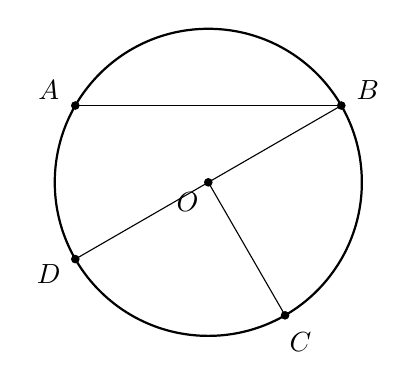
\begin{tikzpicture}[scale=1.3]
  \draw[thick] (0,0) circle (1.5);
  \fill (0,0) circle (1.2pt) node[below left] {$O$};
  \coordinate (A) at (150:1.5); \coordinate (B) at (30:1.5); \coordinate (C) at (-60:1.5); \coordinate (D) at (-150:1.5);
  \draw (A) -- (B); \draw (0,0) -- (C); \draw (B) -- (D);
  \foreach \p/\a in {A/150,B/30,C/-60,D/-150} \fill (\p) circle (1.2pt) node at (\a:1.8) {$\p$};
\end{tikzpicture}
\end{center}

\begin{exercicios}
  \item Indica um raio.
  \item Indica um diâmetro.
  \item Indica uma corda que não seja diâmetro.
  \item Indica um arco.
  \item Qual é a relação entre o diâmetro e o raio?
  \item Qual é a maior corda de uma circunferência?
\end{exercicios}

\secao{Ângulo ao Centro e Ângulo Inscrito}{Calcula a amplitude pedida.}

\begin{center}
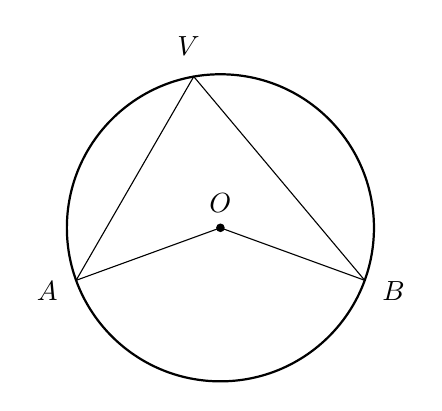
\begin{tikzpicture}[scale=1.3]
  \draw[thick] (0,0) circle (1.5);
  \coordinate (O) at (0,0); \coordinate (A) at (200:1.5); \coordinate (B) at (-20:1.5); \coordinate (V) at (100:1.5);
  \draw (A) -- (O) -- (B); \draw (A) -- (V) -- (B);
  \fill (O) circle (1.2pt) node[above=2pt] {$O$};
  \node at (200:1.8) {$A$}; \node at (-20:1.8) {$B$}; \node at (100:1.8) {$V$};
\end{tikzpicture}
\end{center}

\begin{exercicios}
  \item Se $A\hat{O}B = 140^\circ$, quanto mede o ângulo inscrito $A\hat{V}B$?
  \item Se $A\hat{V}B = 55^\circ$, quanto mede o ângulo ao centro $A\hat{O}B$?
  \item Se o arco $AB$ (que não contém $V$) mede $110^\circ$, quanto mede $A\hat{V}B$?
  \item Um ângulo inscrito mede $38^\circ$. Quanto mede o arco compreendido entre os seus lados?
  \item Quanto mede um ângulo inscrito numa semicircunferência? Justifica.
  \item Dois ângulos inscritos compreendem o mesmo arco. Que relação há entre eles?
  \item Se o ângulo ao centro mede $(3x + 10)^\circ$ e o ângulo inscrito correspondente mede $(x + 25)^\circ$, determina $x$.
  \item O triângulo $AOB$ é isósceles? Justifica. Se $A\hat{O}B = 140^\circ$, quanto mede $O\hat{A}B$?
\end{exercicios}

\secao{Outros Ângulos}{Calcula a amplitude pedida.}
\begin{exercicios}
  \item O ângulo de segmento (formado por uma corda e uma tangente) compreende um arco de $96^\circ$. Quanto mede?
  \item Um ângulo com vértice no interior da circunferência compreende arcos de $80^\circ$ e $40^\circ$. Quanto mede? (Usa a semissoma dos arcos.)
  \item Um ângulo com vértice no exterior da circunferência compreende arcos de $130^\circ$ e $50^\circ$. Quanto mede? (Usa a semidiferença dos arcos.)
  \item Uma reta tangente a uma circunferência é perpendicular a que segmento?
  \item De um ponto $P$ exterior traçam-se duas tangentes à circunferência, que tocam em $T_1$ e $T_2$. Se $T_1\hat{O}T_2 = 120^\circ$, quanto mede $T_1\hat{P}T_2$?
\end{exercicios}

\secao{Polígonos Inscritos}{Resolve.}
\begin{exercicios}
  \item Quanto mede o ângulo ao centro de um pentágono regular inscrito numa circunferência?
  \item Quanto mede o ângulo ao centro de um octógono regular?
  \item Um polígono regular inscrito tem ângulo ao centro de $30^\circ$. Quantos lados tem?
  \item Num quadrilátero inscrito numa circunferência, os ângulos opostos são suplementares. Se $\hat{A} = 75^\circ$ e $\hat{B} = 110^\circ$, determina $\hat{C}$ e $\hat{D}$.
  \item Um quadrilátero $ABCD$ está inscrito numa circunferência e $\hat{A} = 3x$, $\hat{C} = x + 20^\circ$. Determina $x$.
  \item Um hexágono regular está inscrito numa circunferência de raio 5\,cm. Quanto mede o lado? Qual é o perímetro?
  \item Quanto mede cada ângulo interno de um hexágono regular? E de um decágono regular?
\end{exercicios}

\secao{Desafios}{Resolve os problemas.}
\begin{exercicios}
  \item Um triângulo $ABC$ está inscrito numa circunferência e $[AB]$ é um diâmetro. Se $\hat{A} = 35^\circ$, determina $\hat{B}$ e $\hat{C}$.
  \item Os vértices de um triângulo dividem a circunferência em arcos de razão $2:3:4$. Determina os ângulos do triângulo.
  \item Um retângulo está inscrito numa circunferência de raio 5\,cm. Um dos lados mede 6\,cm. Determina a área do retângulo.
  \item Um quadrado está inscrito numa circunferência de raio 4\,cm. Calcula o lado e a área do quadrado.
  \item Explica por que razão um paralelogramo inscrito numa circunferência tem de ser um retângulo.
\end{exercicios}

\end{document}
